\documentclass[review]{siamart190516}

% -----------------------------------------------------------------------------

% 1. Preamble and packages
\usepackage{lipsum}
\usepackage{amsfonts}
\usepackage{amsmath}
\usepackage{graphicx}
\usepackage{subfig}
\usepackage{epstopdf}
\usepackage{hyperref}
\usepackage{algorithmic}
\ifpdf%
  \DeclareGraphicsExtensions{.eps,.pdf,.png,.jpg}
\else
  \DeclareGraphicsExtensions{.eps}
\fi
\usepackage{amsopn}
\DeclareMathOperator{\diag}{diag}
\usepackage{booktabs}

% Paper title
\newcommand{\TheTitle}{%
  Local Fourier Analysis of P-Multigrid for High-Order Finite Element Operators
}

% Short title for running heads (if needed)
\newcommand{\TheShortTitle}{%
  LFA of P-Multigrid for High-Order
}

% Optional PDF information
\ifpdf
\hypersetup{
  pdftitle={\TheTitle},
  pdfauthor={}
}
\fi

% Acknowledge funding or other resources
\newcommand{\TheFunding}{%
  This work is supported by the Exascale Computing Project (17-SC-20-SC), a collaborative effort of two U.S. Department of Energy organizations (Office of Science and the National Nuclear Security Administration) responsible for the planning and preparation of a capable exascale ecosystem, including software, applications, hardware, advanced system engineering and early testbed platforms, in support of the nation’s exascale computing imperative.
}

% Authors: full names plus addresses.
\author{
Jeremy L Thompson\thanks{Department of Applied Mathematics, University of Colorado, Boulder, CO
  (\email{jeremy@jeremylt.org}).}
\and Jed Brown\thanks{Department of Computer Science, University of Colorado, Boulder, CO
  (\email{jed@jedbrown.org}).}
\and Yunhui He\thanks{Department of Mathematics and Statistics, Memorial University of Newfoundland, St. Johns, NL A1C 5S7, Canada
  (\email{yunhui.he@mun.ca}).}
}
\newcommand{\TheShortAuthors}{
J. L. Thompson, J. Brown, and Y. He
}
% Title and funding information on page
\title{{\TheTitle}\thanks{\TheFunding}}
\headers{\TheShortTitle}{\TheShortAuthors}

\begin{document}

\maketitle

\vspace{1cm}

% -----------------------------------------------------------------------------
\begin{abstract}
Multigrid methods are popular for solving linear systems derived from discretizing PDEs.
Local Fourier Analysis (LFA) is a technique for investigating and tuning multigrid methods.
P-multigrid is popular for high-order or spectral finite element methods, especially on unstructured meshes.
In this paper we introduce LFAToolkit.jl, a new Julia package for LFA of high-order finite element methods.
LFAToolkit.jl analyzes preconditioning techniques for arbitrary systems of second order PDEs and supports mixed finite element methods.
Specifically, in this paper we develop LFA of p-multigrid with arbitrary second-order PDEs using high-order finite element discretizations and investigate tuning Jacobi and Chebyshev smoothing for two-grid schemes.
Traditional estimates of the optimal Jacobi smoothing parameter are ill-suited to p-multigrid for high-order elements, but analysis of the two-grid smoothing factor can provide a reasonable underestimate of the optimal Jacobi smoothing parameter for multigrid schemes.
\end{abstract}
% -----------------------------------------------------------------------------

% -----------------------------------------------------------------------------
\begin{keywords}
  % Keywords that describe the paper
  local fourier analysis, p-multigrid, high-order, finite elements
\end{keywords}
% -----------------------------------------------------------------------------

% -----------------------------------------------------------------------------
\section{Introduction}\label{sec:intro}
% -----------------------------------------------------------------------------

Multigrid methods \cite{brandt1982guide, briggs2000multigrid, stuben1982multigrid} are popular for solving linear systems derived from descretizing PDEs.
Local Fourier Analysis (LFA) \cite{brandt1977multi, wienands2004practical} is a powerful tool for investigating and tuning multigrid methods.

High-order finite element methods offer advantages over low-order finite elements \cite{demkowicz1989toward, oden1989toward, rachowicz1989toward}; however, high-order finite elements are less common because a linear operator or the Jacobian of a non-linear operator rapidly loses sparsity in a sparse matrix representation.
Matrix-free formulations of these methods, such as described in \cite{brown2010efficient, knoll2004jacobian}, provide efficient implementations of these methods on modern hardware \cite{libceed-user-manual, fischer2020scalability}.
LFA of h-multigrid with high-order finite elements was developed in \cite{he2020two} for Lagrange bases with uniformly spaced nodes.

P-multigrid, developed by R{\o}nquist and Patera \cite{ronquist1987spectral}, is based on decreasing the order of the bases in high-order or spectral finite element methods rather than aggregating elements to coarsen the mesh. While it is possible \cite{davydov2019matrix} to use high-order finite element methods with matrix-free implementation of h-multigrid preconditioning on complex problems, p-multigrid can be a more natural fit for high-order methods on unstructured meshes.

In this paper, we develop LFA of p-multigrid with arbitrary second-order PDEs using high-order finite element discretizations and investigate Jacobi and Chebyshev smoothing for two-grid schemes with LFAToolkit.jl \cite{thompson2021toolkit}, a new Julia package for LFA of high-order finite element methods..

We investigate tuning Jacobi and Chebyshev smoothing on the one and two dimensional Laplacian and three dimensional Neo-Hookean hyperelasticity.
Traditional estimates of the optimal Jacobi smoothing parameter are ill-suited to p-multigrid for high-order elements.

This paper is organized as follows.
In Section \ref{sec:notation} we outline the notation for LFA used in this paper.
In Section \ref{sec:lfa} we develop the notation for LFA of second-order PDEs with arbitrary order bases, dimension, and number of components used in LFAToolkit.jl and we use this notation to develop LFA of p-multigrid as well as Jacobi and Chebyshev smoothers.
Section \ref{sec:results} contains numerical results investigating the performance of Jacobi smoothing for p-multigrid on the one and two dimensional Laplacian and three dimensional Neo-Hookean hyperelasticity, and Section \ref{sec:conclusion} contains concluding remarks. 

% -----------------------------------------------------------------------------
\subsection{Reproducibility}\label{sec:reproducibility}
% -----------------------------------------------------------------------------

The numerical results in this paper were generated using the Julia package LFAToolkit.jl \cite{thompson2021toolkit}.
This package is under active development and may be found on GitHub at \href{https://github.com/jeremylt/LFAToolkit.jl}{jeremylt/LFAToolkit.jl}.
This repository contains Julia scripts and interactive Jupyter notebooks that can replicate the tables and plots in this paper.

% -----------------------------------------------------------------------------
\section{Definitions and Notation}\label{sec:notation}
% -----------------------------------------------------------------------------

In this section, we introduce the notation required to describe LFA.

Consider a scalar Toeplitz operator $L_h$ on an infinite one dimensional uniform grid $G_h$,
\begin{equation}
\begin{split}
L_h \mathrel{\hat{=}} \left[ s_\kappa \right]_h \left( \kappa \in V \right)\\
L_h w_h \left( x \right) = \sum_{\kappa \in V} s_\kappa w_h \left( x + \kappa h \right)
\end{split}
\end{equation}
where $V \subset \mathbb{Z}$ is a finite index set, $s_\kappa \in \mathbb{R}$ are constant coefficients, and $w_h \left( x \right)$ is a $l^2$ function on $G_h$.

Since $L_h$ is Toeplitz, it can be diagonalized by the standard Fourier modes $\varphi \left( \theta, x \right) = e^{\imath \theta x / h}$.

\begin{definition}[Symbol of $L_h$]\label{def:symbol}
If for all grid functions $\varphi \left( \theta, x \right)$ we have
\begin{equation}
L_h \varphi \left( \theta, x \right) = \tilde{L}_h \left( \theta \right) \varphi \left( \theta, x \right)
\end{equation}
then we define $\tilde{L}_h \left( \theta \right) = \sum_{\kappa \in V} s_\kappa e^{\imath \theta \kappa}$ as the symbol of $L_h$.
\end{definition}

This definition can be extended to a $p \times p$ linear system of operators by
\begin{equation}
\tilde{\mathbf{L}}_h =
\begin{bmatrix}
    \tilde{L}_h^{1, 1} && \cdots && \tilde{L}_h^{1, p} \\
    \vdots             && \vdots && \vdots             \\
    \tilde{L}_h^{p, 1} && \cdots && \tilde{L}_h^{p, p} \\
\end{bmatrix}
\end{equation}
where $\tilde{L}_h^{i, j}$, $i, j \in \left[1, 2, \dots, p \right]$ is given by scalar Toeplitz operators describing how component $j$ appears in the equation for component $i$.

For a system of equations representing an error propagation operator in a relaxation scheme, the spectral radius of the symbol matrix determines now rapidly the scheme decreases error at a target frequency.
Low frequencies are given by $\theta \in T^{\text{low}} = \left[ - \pi / 2, \pi / 2 \right)$ and high frequencies are given by $\theta \in T^{\text{high}} = \left[ - \pi / 2, 3 \pi / 2 \right) \setminus T^{\text{low}}$. % TODO: or be honest and call it [-\pi, \pi) \setminus T^{\text{low}}

% -----------------------------------------------------------------------------
\section{Local Fourier Analysis for P-Multigrid}\label{sec:lfa}
% -----------------------------------------------------------------------------

We now develop the LFA formulation used in LFAToolkit.jl, first in 1 dimension and then in multiple dimensions, followed by LFA of polynomial smoothers and LFA of p-multigrid with high-order finite elements.

% -----------------------------------------------------------------------------
\subsection{High-Order Finite Elements}\label{sec:highorder}
% -----------------------------------------------------------------------------

We will use the representation of the weak form of linear second-order PDEs described in \cite{brown2010efficient}, which is given by
\begin{equation}
\langle v, f \left( u \right) \rangle = \int_{\Omega}
\begin{bmatrix}
  v^T & \nabla v^T    \\
\end{bmatrix}
\begin{bmatrix}
  f_{0, 0} & f_{0, 1} \\
  f_{1, 0} & f_{1, 1} \\
\end{bmatrix}
\begin{bmatrix}
  u                   \\
  \nabla u            \\
\end{bmatrix}
= \int_{\Omega} f v, \forall v \in V
\end{equation}
for some suitable $V \subseteq H_0^1 \left( \Omega \right)$.
In this equation, $f_{i, j}$ may come from a linear PDE or the linearization of a non-linear problem.
Boundary terms have been omitted, as they are not present on the infinite uniform grid $G_h$.

Selecting a finite element basis, we can discretize this weak form and produce
\begin{equation}\label{pdediscrete}
\mathbf{A} \mathbf{u} = \mathbf{b}.
\end{equation}

Using the algebraic representation of PDE operators given in \cite{brown2010efficient}, the PDE operator $A$ is of the form
\begin{equation}\label{efficienthighorder}
\begin{split}
\mathbf{A} = \mathbf{P}^T \mathbf{A}_e \mathbf{P}\\
\mathbf{A}_e = \mathbf{B}^T \mathbf{D} \mathbf{B}
\end{split}
\end{equation}
where $\mathbf{P}$ represents the element assembly operator, $\mathbf{B}$ is a basis operator which computes the values and derivatives of the basis functions at the quadrature points, and $\mathbf{D}$ is a block diagonal operator which provides the pointwise application of the bilinear form on the quadrature points, to include quadrature weights and the change in coordinates between the physical and reference space.

Consider the specific case of a Topeliz operator representing an arbitrary second order scalar PDE in 1D with basis of polynomial order $p$ given in the form of Equations \ref{pdediscrete} and \ref{efficienthighorder}.
The nodes on the left and right boundaries of the element map to the same Fourier mode due to periodicity, so we can compute the symbol matrix as
\begin{equation}\label{symbolscalar1d}
\tilde{\mathbf{A}} = \mathbf{Q}^T \left( \mathbf{A}_e \odot \left[ e^{\imath \left( x_i - x_j \right) \theta / h} \right] \right) \mathbf{Q}
\end{equation}
where $\odot$ represents pointwise multiplication of the elements, $h$ is the length of the element, and $i, j \in \left[ 0, 1, \dots, p\right]$.
$\mathbf{Q}$ is a $\left( p + 1 \right) \times p$ matrix that localizes Fourier modes to each element.
\begin{equation}
\mathbf{Q} =
\begin{bmatrix}
    \mathbf{I}   \\
    \mathbf{e}_0 \\
\end{bmatrix} =
\begin{bmatrix}
    1      && 0      && \cdots && 0      \\
    0      && 1      && \cdots && 0      \\
    \vdots && \vdots && \vdots && \vdots \\
    0      && 0      && \cdots && 1      \\
    1      && 0      && \cdots && 0      \\
\end{bmatrix}
\end{equation}

The computation of this symbol matrix extends to more complex PDE with multiple components and in higher dimensions.

Multiple components are supported by extending the $p \times p$ system of Toeplitz operators in Equation \ref{symbolscalar1d} to a $\left( p \cdot ncomp \right) \times \left( p \cdot ncomp \right)$ system of operators.

The infinite uniform grid $G_h$ is extended into higher dimensions by taking the direct sum of the one dimensional grid.
Tensor product are used to extend the one dimensional bases into higher dimensions.
The basis evaluation operators in two dimensions are given by
\begin{equation}
\begin{split}
\mathbf{B}_{\text{interp2d}} = \mathbf{B}_{\text{interp1d}} \otimes \mathbf{B}_{\text{interp1d}} \\
\mathbf{B}_{\text{grad2d}} =
\begin{bmatrix}
    \mathbf{B}_{\text{grad1d}} \otimes \mathbf{B}_{\text{interp1d}} \\
    \mathbf{B}_{\text{interp1d}} \otimes \mathbf{B}_{\text{grad1d}} \\
\end{bmatrix}.
\end{split}
\end{equation}

In a similar fashion, the localization operator for Fourier modes in two dimensions is given by
\begin{equation}
\mathbf{Q}_{\text{2d}} = \mathbf{Q} \otimes \mathbf{Q}.
\end{equation}
As with tensor product bases, an analogous computation can be done in higher dimensions.

\begin{definition}
The symbol matrix of a finite element operator for an arbitrary second order PDE with any number of components, basis order, and dimension is given by
\begin{equation}\label{symbolhighorder}
\tilde{\mathbf{A}} = \mathbf{Q}^T \left( \mathbf{A}_e \odot \left[ e^{\imath \sum_d \left( \mathbf{x}_i - \mathbf{x}_j \right) \mathbf{\theta} / \mathbf{h}} \right] \right) \mathbf{Q}
\end{equation}
where $\odot$ represents pointwise multiplication of the elements, $\mathbf{h}$ is the length of the element in each dimension, $\mathbf{\theta}$ is the target frequency in each dimension, and $i, j \in \left[ 0, 1, \dots, p\right]$.
$\mathbf{A}_e$ is the finite element operator for the element and $\mathbf{Q}$ is the localization of Fourier modes on an element.
\end{definition}\label{def:high_order_symbol}

Note that this LFA notation is applicable to any second-order PDE with a weak form that can be represented by Equation \ref{efficienthighorder}.
This representation is used in LFAToolkit.jl, where the users provide the finite element basis $\mathbf{B}$, the node to mode mapping $\mathbf{Q}$, and the pointwise representation of the weak form $\mathbf{D}$, and the software can provide the LFA of the PDE with various preconditioners.

% -----------------------------------------------------------------------------
\subsection{Polynomial Smoothers}\label{sec:smooth}
% -----------------------------------------------------------------------------

Multigrid methods require a fine grid smoother, typically appled both before and after the coarse grid correction is computed.
In this section, we compute the error propegation operator for two polynomial smoothers, Jacobi and Chebyshev.

The error propagation operator for a smoother is given by $\mathbf{S} = \mathbf{I} - \mathbf{M}^{-1} \mathbf{A}$, where $\mathbf{M}^{-1}$ is given by the particular smoother under investigation.

% -----------------------------------------------------------------------------
\subsubsection{Jacobi Smoother}\label{sec:jacobi}
% -----------------------------------------------------------------------------

Following the derivation from Section \ref{sec:highorder}, the symbol of the Jacobi error propagation operator is given by
\begin{equation}
\tilde{\mathbf{S}} \left( \omega, \theta \right) = \mathbf{I} - \tilde{\mathbf{M}}^{-1} \left( \theta \right) \tilde{\mathbf{A}} \left( \theta \right) = \mathbf{I} - \left( \mathbf{Q}^T \diag \left( \mathbf{A}_e \right) \mathbf{Q} \right)^{-1} \tilde{\mathbf{A}} \left( \theta \right),
\end{equation}
where this expression has been simplified by the fact that $e^{\imath \left( x_i - x_i \right) \theta / h} = 1$.

If multiple pre or post-smoothing passes are used by our multigrid algorithm, we take the product of the symbol matrix with itself to represent repeated application.

\begin{definition}
The symbol of the error propagation operator for Jacobi smoothing is given by
\begin{equation}
\tilde{\mathbf{S}} \left( \nu, \omega, \theta \right) = \left( \mathbf{I} - \left( \mathbf{Q}^T \diag \left( \mathbf{A}_e \right) \mathbf{Q} \right)^{-1} \tilde{\mathbf{A}} \left( \theta \right) \right)^\nu,
\end{equation}
where $\nu$ is the number of smoothing passes.
\end{definition}\label{def:jacobi_symbol}

\begin{figure}[!tbp]
  \centering
  \subfloat[Spectrum of Jacobi for $p = 4$]{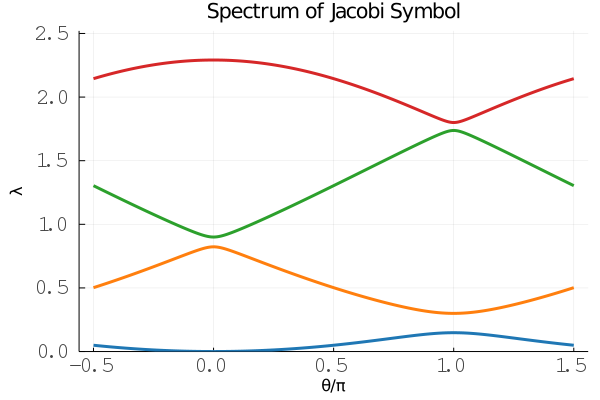
\includegraphics[width=0.48\textwidth]{img/jacobi_spectrum_5}\label{fig:jacobi_spectrum}}
  \hfill
  \subfloat[Smoothing Factor of Jacobi for $p = 4$]{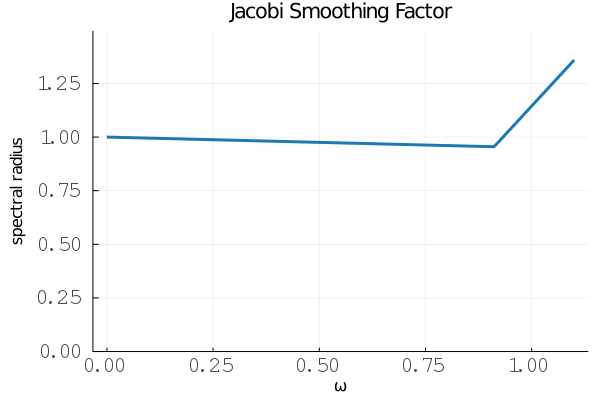
\includegraphics[width=0.48\textwidth]{img/jacobi_smoothing_5}\label{fig:jacobi_smooth_factor}}
  \caption{Jacobi smoothing for high-order finite elements}
\end{figure}

Using Definition \ref{def:jacobi_symbol}, we plot the eigenvalues of $\tilde{\mathbf{M}}^{-1} \tilde{\mathbf{A}} \left( \theta \right)$ in Figure \ref{fig:jacobi_spectrum} for the one dimensional Laplacian with a 4th order H1 Lagrange basis on Gauss-Lobatto points.
In Figure \ref{fig:jacobi_smooth_factor} we plot the LFA predicted smoothing factor for Jacobi smoothing as a function of the smoothing parameter $\omega$.
The Jacobi smoothing factor is not an accurate predictor of the two-grid performance, as we will see below.

% -----------------------------------------------------------------------------
\subsubsection{Chebyshev Smoother}\label{sec:chebyshev}
% -----------------------------------------------------------------------------

It is well known that polynomial smoothers allow more aggressive coarsening than Jacobi \cite{brannick2015polynomial}.
For further discussion of the error propagation properties of the Chebyshev semi-iterative method, see \cite{gutknecht2002revisited}.

We use the Jacobi preconditioned operator, $\left( \diag {\mathbf{A}} \right)^{-1} {\mathbf{A}}$, in this iteration instead of the finite element operator ${\mathbf{A}}$, similar to the discussion in \cite{adams2003parallel}.

The terms in the Chebyshev semi-iterative method can be modeled by the three term recurrence relation given by
\begin{equation}
\mathbf{x}_{n + 1} = - \left( \mathbf{r}_n + \alpha \mathbf{x}_n + \beta_{n - 1} \mathbf{x}_{n - 1} \right) / \gamma_{n - 1}
\label{eq:chebyshev_recursive}
\end{equation}
where the spectrum of $\left( \diag {\mathbf{A}} \right)^{-1} {\mathbf{A}}$ lies on the line segment $\left[ \alpha - c, \alpha + c \right]$ and the parameters $\beta$ and $\gamma$ are given by the recurrence
\begin{equation}
\begin{tabular}{c c}
$\beta_0 = - \frac{c^2}{2 \alpha}$ & $\gamma_0 = - \alpha$\\
$\beta_n = \frac{c}{2} \frac{T_n \left( \eta \right)}{T_{n + 1} \left( \eta \right)} = \left( \frac{c}{2} \right)^2 \frac{1}{\gamma_n}$ & $\gamma_n = \frac{c}{2} \frac{T_{n + 1} \left( \eta \right)}{T_n \left( \eta \right)} = - \left( \alpha + \beta_{n - 1} \right)$.
\end{tabular}
\end{equation}
In this equation, $T_i \left( \zeta \right) = 2 \zeta T_{i - 1} \left( \zeta \right) - T_{i - 2} \left( \zeta \right)$ are the classical Chebyshev polynomials, which are evaluated at the point $\eta = - \alpha / c$.

The residual in the Chebyshev semi-iterative method can therefore be modeled by the three term recurrence
\begin{equation}
\mathbf{r}_{n + 1} = \left( \left( \diag {\mathbf{A}} \right)^{-1} {\mathbf{A}} \mathbf{r}_n - \alpha \mathbf{r}_n - \beta_{n - 1} \mathbf{r}_{n - 1} \right) / \gamma_{n - 1}.
\label{eq:chebyshev_error_recursive}
\end{equation}

Using the recurrence relation given in Equation \ref{eq:chebyshev_error_recursive}, we can define the error propagation of the $n$th order Chebyshev smoother in terms of the error in the first term:
\begin{equation}
\begin{tabular}{c}
$\mathbf{E}_0 = \mathbf{I}$\\
$\mathbf{E}_1 = \mathbf{I} - \alpha \left( \diag {\mathbf{A}} \right)^{-1} {\mathbf{A}}$\\
$\mathbf{E}_n = \left( \alpha \mathbf{E}_{n - 1} + \beta_{n - 2} \mathbf{E}_{n - 2} - \left( \diag {\mathbf{A}} \right)^{-1} {\mathbf{A}} \mathbf{E}_{n - 2} \right) / \gamma_{n - 1}$
\end{tabular}
\label{eq:chebyshev_error_propagation}
\end{equation}
With this recursive definition of the error propagation operator, we can define the symbol for Chebyshev smoothing.

\begin{definition}
The symbol of the error propagation operator for a $n$th order Chebyshev smoother based on the Jacobi preconditioned operator is given by
\begin{equation}
\tilde{\mathbf{S}} \left( \nu, n, \theta \right) = \left( \tilde{\mathbf{E}}_n \right)^\nu,
\end{equation}
where $\nu$ is the number of smoothing passes and $\tilde{\mathbf{E}}_n \left( \mathbf{\theta} \right)$ is given by the recursive definition
\begin{equation}
\begin{tabular}{c}
$\tilde{\mathbf{E}}_0 \left( \mathbf{\theta} \right) = \mathbf{I}$\\
$\tilde{\mathbf{E}}_1 \left( \mathbf{\theta} \right) = \mathbf{I} - \alpha \tilde{\mathbf{A}}_J \tilde{\mathbf{A}} \left( \mathbf{\theta} \right)$\\
$\tilde{\mathbf{E}}_n \left( \mathbf{\theta} \right) = \left( \alpha \tilde{\mathbf{E}}_{n - 1} \left( \mathbf{\theta} \right) + \beta_{n - 2} \tilde{\mathbf{E}}_{n - 2} \left( \mathbf{\theta} \right) - \tilde{\mathbf{A}}_J \tilde{\mathbf{A}} \left( \mathbf{\theta} \right) \tilde{\mathbf{E}}_{n - 2} \left( \mathbf{\theta} \right) \right) / \gamma_{n - 1}$
\end{tabular}
\end{equation}
\label{def:chebyshev_symbol}
\end{definition}
with $\tilde{\mathbf{A}}_J = \left( \mathbf{Q}^T \diag \left( \mathbf{A}_e \right) \mathbf{Q} \right)^{-1}$ giving the symbol of the Jacobi smoother.

\begin{figure}[!tbp]
  \centering
  \subfloat[Spectrum of Chebyshev for $p = 4$]{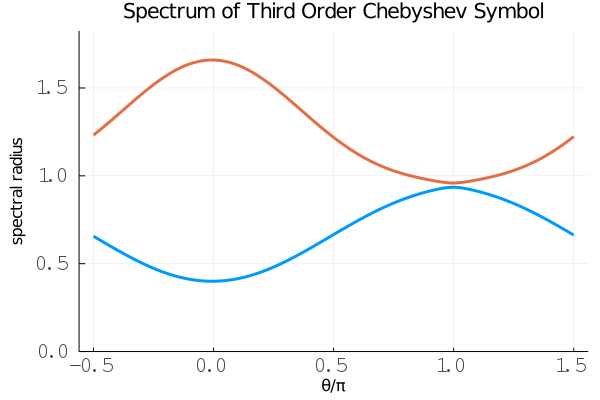
\includegraphics[width=0.48\textwidth]{img/chebyshev_spectrum_5}\label{fig:chebyshev_spectrum}}
  \hfill
  \subfloat[Smoothing Factor of Chebyshev for $p = 4$]{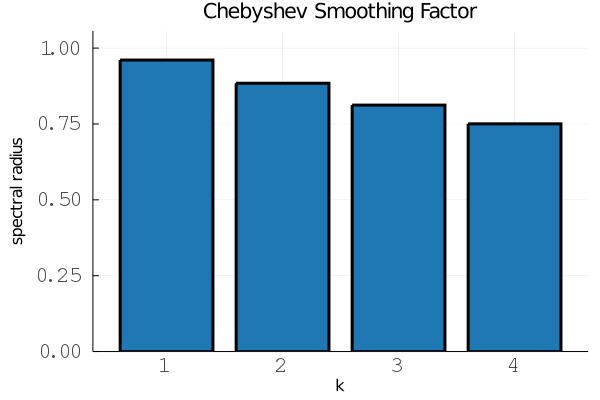
\includegraphics[width=0.48\textwidth]{img/chebyshev_smoothing_5}\label{fig:chebyshev_smooth_factor}}
  \caption{Chebyshev smoothing for high-order finite elements}
\end{figure}

Using Definition \ref{def:chebyshev_symbol}, we plot the eigenvalues of $\tilde{\mathbf{M}}^{-1} \tilde{\mathbf{A}} \left( \theta \right)$ in Figure \ref{fig:chebyshev_spectrum} for the one dimensional Laplacian with a 4th order H1 Lagrange basis on Gauss-Lobatto points.
In Figure \ref{fig:chebyshev_smooth_factor} we plot the LFA predicted smoothing factor for Chebyshev smoothing as a function of the polynomial order, $\omega$.

% -----------------------------------------------------------------------------
\subsection{P-Multigrid}\label{sec:multigrid}
% -----------------------------------------------------------------------------

With this representation of the symbol of high-order PDE operators, we can derive the symbol of the p-multigrid error propagation operator.

The total multigrid error propagation operator is given by
\begin{equation}
\mathbf{E}_{\text{TMG}} = \mathbf{S}_f \left( \mathbf{I} - \mathbf{P}_{\text{ctof}} \mathbf{A}_c^{-1} \mathbf{R}_{\text{ftoc}} \mathbf{A}_f \right) \mathbf{S}_f
\end{equation}
where $\mathbf{S}_f$ represents the smoother error propagation operator, while $\mathbf{P}_{\text{ctof}}$ and $\mathbf{R}_{\text{ftoc}}$ represent the grid prolongation and restriction operators, respectively.
Some multigrid implementations allow the number of pre and post smoothing passes to be set independently.
This derivation of LFA for p-multigrid allows independently setting these parameters; however we omit this in the notation for simplicity.

This error propagation operator can represent both h-multigrid and p-multigrid, depending upon the grid transfer operators and coarse grid representation chosen, but we focus on p-multigrid grid transfer operators in this paper.

% -----------------------------------------------------------------------------
\subsubsection{Grid Transfer Operator}\label{sec:grids}
% -----------------------------------------------------------------------------

In p-multigrid, grid transfer operators can be represented elementwise and can thus be easily represented in the form of Equation \ref{efficienthighorder}.
The prolongation operator from the coarse to the fine grid can be represented by
\begin{equation}
\begin{split}
\mathbf{P}_{\text{ctof}} = \mathbf{P}_f^T \mathbf{P}_e \mathbf{P}_c\\
\mathbf{P}_e = \mathbf{I} \mathbf{D}_{\text{scale}} \mathbf{B}_{\text{ctof}}
\end{split}
\end{equation}
where $\mathbf{B}_{ctof}$ is an interpolation operator from the coarse grid basis to the fine grid basis, $\mathbf{P}_f$ is the fine grid element assembly operator, $\mathbf{P}_c$ is the coarse grid element assembly operator, and $\mathbf{D}_{\text{scale}}$ is a scaling operator to account for node multiplicity across element interfaces.
Restriction from the fine grid to the coarse grid is given by the transpose, $\mathbf{R}_{\text{ftoc}} = \mathbf{P}_{\text{ctof}}^T$.

Following the derivation from Section \ref{sec:highorder}, we can derive the symbols of $\mathbf{P}_{\text{ctof}}$ and $\mathbf{R}_{\text{ftoc}}$.

\begin{definition}
The symbol of the p-prolongation is given by
\begin{equation}
\tilde{\mathbf{P}}_{\text{ctof}} \left( \theta \right) = \mathbf{Q}_f^T \left( \mathbf{P}_e \odot \left[ e^{\imath \sum_d \left( \mathbf{x}_{i, f} - \mathbf{x}_{j, c} \right) \mathbf{\theta} / \mathbf{h}} \right] \right) \mathbf{Q}_c
\end{equation}
where $i \in \left[ 0, 1, \dots, p_{\text{fine}} \right]$, $\mathbf{h}$ is the length of the element, and $j \in \left[ 0, 1, \dots, p_{\text{coarse}} \right]$.
The matrices $\mathbf{Q}_f$ and $\mathbf{Q}_c$ are the localization mappings for the fine and coarse grid, respectively, and the element p-prolongation operator is given by $\mathbf{P}_e = \mathbf{D}_{\text{scale}} \mathbf{B}_{\text{ctof}}$.
\end{definition}\label{def:prolongation_symbol}

\begin{definition}
The symbol of p-restriction is given by the expression
\begin{equation}
\tilde{\mathbf{R}}_{\text{ftoc}} \left( \theta \right) = \mathbf{Q}_c^T \left( \mathbf{R}_e \odot \left[ e^{\imath \sum_d \left( \mathbf{x}_{i, c} - \mathbf{x}_{j, f} \right) \mathbf{\theta} / \mathbf{h}} \right] \right) \mathbf{Q}_f
\end{equation}
where $i \in \left[ 0, 1, \dots, p_{\text{coarse}} \right]$, $\mathbf{h}$ is the length of the element, and $j \in \left[ 0, 1, \dots, p_{\text{fine}} \right]$.
The matrices $\mathbf{Q}_f$ and $\mathbf{Q}_c$ are the localization mappings for the fine and coarse grid, respectively, and the element p-restriction operator is given by $\mathbf{R}_e = \mathbf{P}_e^T = \mathbf{B}_{\text{ctof}}^T \mathbf{D}_{\text{scale}}$.
\end{definition}\label{def:restriction_symbol}

% -----------------------------------------------------------------------------
\subsubsection{Multigrid Error Propagation Symbol}\label{sec:multigridsymbol}
% -----------------------------------------------------------------------------

We can combine these expressions to give the symbol of the error propagation operator.

\begin{definition}
The symbol for the p-multgrid error propagation operator is given by
\begin{equation}
\tilde{\mathbf{E}}_{\text{TMG}} \left( \nu, \omega, \theta \right) = \tilde{\mathbf{S}}_f \left( \nu, \omega, \theta \right) \left[ \mathbf{I} - \tilde{\mathbf{P}}_{\text{ctof}} \left( \theta \right) \tilde{\mathbf{A}}_c^{-1} \left( \theta \right) \tilde{\mathbf{R}}_{\text{ftoc}} \left( \theta \right) \tilde{\mathbf{A}}_f \left( \theta \right) \right] \tilde{\mathbf{S}}_f \left( \nu, \omega, \theta \right).
\end{equation}
\end{definition}\label{def:pmultigrid_symbol}

Note again that this derivation is applicable for any PDE with a weak form that can be represented by Equation \ref{efficienthighorder}.
This expression can be extended to represent multi-level schemes by recursively applying $\tilde{\mathbf{M}}_{\text{TMG}}$ until the coarsest grid is reached.

% -----------------------------------------------------------------------------
\section{Numerical Results}\label{sec:results}
% -----------------------------------------------------------------------------

In this section, we present numerical results for this analysis for the scalar Laplacian in one and two dimensions and Neo-Hookean hyperelasticity in three dimensions with H1 Lagrange bases on Gauss-Lobatto points with Gauss-Legendre quadrature.

% -----------------------------------------------------------------------------
\subsection{Scalar Lapalcian - 1D Convergence Factors}\label{sec:1dresults}
% -----------------------------------------------------------------------------

\subsubsection{Jacobi Smoothing}
% -----------------------------------------------------------------------------

\begin{figure}[!tbp]
  \centering
    \subfloat[Convergence for $p = 4$ to $p = 2$, $\nu = 1$]{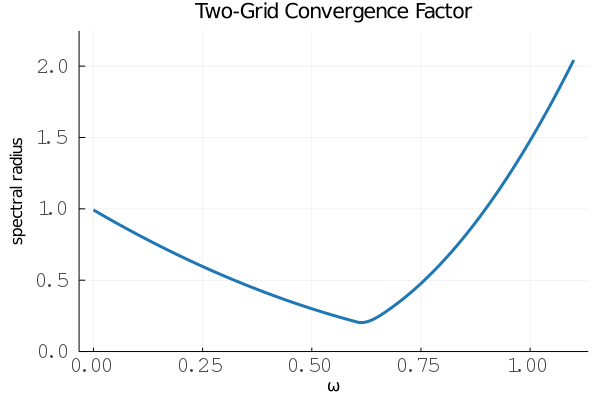
\includegraphics[width=0.48\textwidth]{img/two_grid_converge_5_to_3}\label{fig:two_grid_5_3}}
    \subfloat[Convergence for $p = 4$ to $p = 1$, $\nu = 1$]{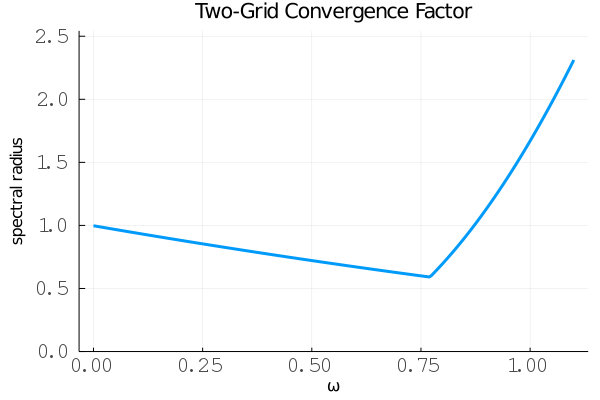
\includegraphics[width=0.48\textwidth]{img/two_grid_converge_5_to_2}\label{fig:two_grid_5_2}} \\
    \subfloat[Convergence for $p = 4$ to $p = 2$, $\nu = 2$]{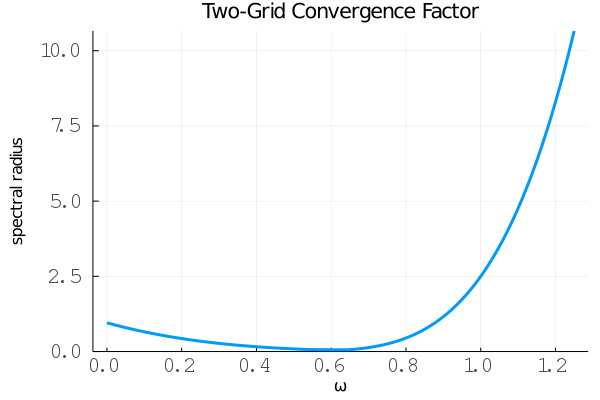
\includegraphics[width=0.48\textwidth]{img/two_grid_converge_5_to_3_2smooth}\label{fig:two_grid_5_3_2smooth}}
    \subfloat[Convergence for $p = 4$ to $p = 1$, $\nu = 2$]{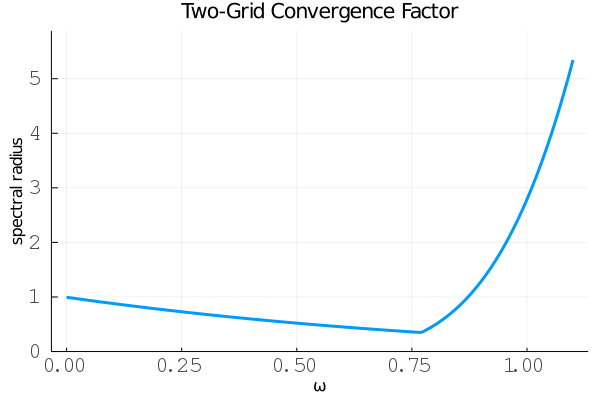
\includegraphics[width=0.48\textwidth]{img/two_grid_converge_5_to_2_2smooth}\label{fig:two_grid_5_2_2smooth}} \\
  \caption{Two-grid analysis for Jacobi smoothing for high-order finite elements}
\end{figure}

In Figures \ref{fig:two_grid_5_3} and \ref{fig:two_grid_5_2} we plot the two-grid convergence factor for p-multigrid with a single iteration of Jacobi pre and post-smoothing for the one dimensional Laplacian as a function of the Jacobi smoothing parameter $\omega$,
and in Figures \ref{fig:two_grid_5_3_2smooth} and \ref{fig:two_grid_5_2_2smooth} we plot the two-grid convergence factor for p-multigrid with two iterations of Jacobi pre and post-smoothing for the one dimensional Laplacian as a function of the Jacobi smoothing parameter $\omega$.
On the left we show conservative coarsening from quartic to quadratic elements and on the right we show more aggressive coarsening from quartic to linear elements.
As expected, the two-grid convergence factor decreases as we coarsen more rapidly.
Also, the effect of underestimating the optimal Jacobi smoothing parameter, $\omega$, is less pronounced than the effect of overestimating the smoothing parameter, especially with a higher number of pre and post-smooths.

In contrast to the previous work on h-multigrid for high-order finite elements, \cite{he2020two}, poorly chosen values of $\omega < 1.0$ can result in a spectral radius of the p-multigrid error propagation symbol that is greater than $1$, indicating that application of p-multigrid with Jacobi smoothing at these parameter values will result in increased error.

\begin{table}[ht!]
\begin{center}
\begin{tabular}{l cc cc cc}
  \toprule
  $p_{\text{fine}}$ to $p_{\text{coarse}}$  &  \multicolumn{2}{c}{$\nu = 1$}          &  \multicolumn{2}{c}{$\nu = 2$}          &  \multicolumn{2}{c}{$\nu = 3$}          \\
  %\cmidrule(lr){2-3} \cmidrule(lr){4-5} \cmidrule(lr){6-7}
                                            &  $\rho_{\min}$ & $\omega_{\text{opt}}$  &  $\rho_{\min}$ & $\omega_{\text{opt}}$  &  $\rho_{\min}$ & $\omega_{\text{opt}}$  \\
  \midrule
  $p = 2$ to $p = 1$          &  0.132 & 0.636  &  0.060 & 0.689  &  0.041 & 0.717   \\
  %\midrule
  $p = 4$ to $p = 2$          &  0.203 & 0.615  &  0.059 & 0.640  &  0.045 & 0.701   \\
  $p = 4$ to $p = 1$          &  0.591 & 0.771  &  0.349 & 0.771  &  0.206 & 0.771   \\
  %\midrule
  $p = 8$ to $p = 4$          &  0.249 & 0.602  &  0.068 & 0.601  &  0.033 & 0.633   \\
  $p = 8$ to $p = 2$          &  0.666 & 0.735  &  0.444 & 0.735  &  0.296 & 0.735   \\
  $p = 8$ to $p = 1$          &  0.874 & 0.783  &  0.763 & 0.783  &  0.667 & 0.783   \\
  %\midrule
  $p = 16$ to $p = 8$         &  0.294 & 0.577  &  0.087 & 0.576  &  0.034 & 0.587   \\
  $p = 16$ to $p = 4$         &  0.718 & 0.692  &  0.516 & 0.692  &  0.371 & 0.692   \\
  $p = 16$ to $p = 2$         &  0.906 & 0.731  &  0.820 & 0.731  &  0.743 & 0.731   \\
  $p = 16$ to $p = 1$         &  0.967 & 0.743  &  0.936 & 0.743  &  0.906 & 0.743   \\
  \bottomrule
\end{tabular}
\end{center}
\caption{Two-grid smoothing factor and optimal Jacobi parameter for 1D Laplacian}
\label{table:two_grid_1d}
\end{table}

The results in Table \ref{table:two_grid_1d} provide the minimal LFA smoothing factor and optimal values of $\omega$ for two-grid high-order p-multigrid for a variety of polynomial orders and coarsening factors.

\begin{figure}[!tbp]
  \centering
    \subfloat[Convergence for $p = 4$ to $p = 1$, $\nu = 2$]{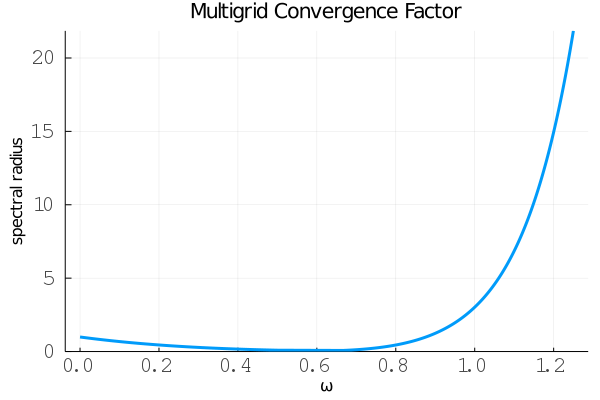
\includegraphics[width=0.48\textwidth]{img/multi_grid_converge_5_to_2_2smooth}\label{fig:multi_grid_5_2_2smooth}}
    \subfloat[Convergence for $p = 8$ to $p = 1$, $\nu = 2$]{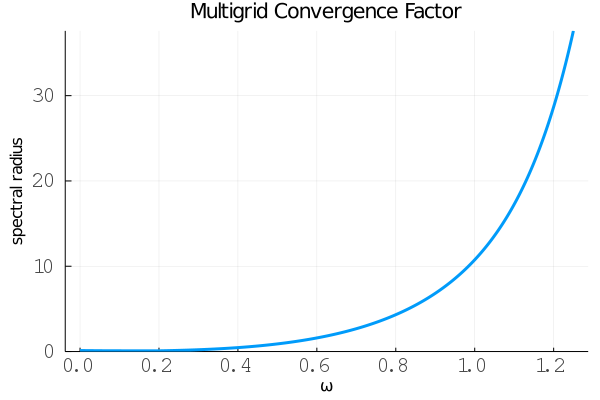
\includegraphics[width=0.48\textwidth]{img/multi_grid_converge_9_to_2_2smooth}\label{fig:multi_grid_9_2_2smooth}}
  \caption{Multigrid analysis for Jacobi smoothing for high-order finite elements}
\end{figure}

In Figures \ref{fig:multi_grid_5_2_2smooth} and \ref{fig:multi_grid_9_2_2smooth} we plot the multigrid convergence factor for p-multigrid with two iterations of Jacobi pre and post-smoothing for the one dimensional Laplacian as a function of the Jacobi smoothing parameter $\omega$.
From this chart, we can see that the additional Jacobi iterations increase the amplification of the error in the full multigrid scheme for poorly chosen values of $\omega$.

For low order h-multigrid, the classical estimate of the optimal Jacobi smoothing parameter is given by $\omega = 2 / \left( \lambda_{\text{max, high}} + \lambda_{\text{min, high}} \right)$, where $\lambda_{\text{max, high}}$ and $\lambda_{\text{min, high}}$ are the maximum and minimum eigenvalues of $\tilde{S}_f \left( \theta \right)$ for $\theta \in T^{\text{high}}$.
The modified estimate from \cite{he2020two} for h-multigrid for high-order finite elements is given by $\omega = 2 / \left( \lambda_{\text{max}} + \lambda_{\text{min, high}} \right)$, where $\lambda_{\text{max}}$ is the maximum eigenvalue of $\tilde{S}_f \left( \theta \right)$ for $\theta \in T^{\text{low}} \cup T^{\text{high}}$.
Both of these estimates result in values of $\omega$ that increase the iterate error.

Optimal parameter estimation is an open question for high-order p-multigrid, but optimization techniques, such as those discussed in \cite{brown2021tuning}, can be used to tune these parameters, especially for more complex PDEs.

\subsubsection{Chebyshev Smoothing}
% -----------------------------------------------------------------------------

\begin{figure}[!tbp]
  \centering
    \subfloat[Convergence for $p = 4$ to $p = 2$, $\nu = 1$]{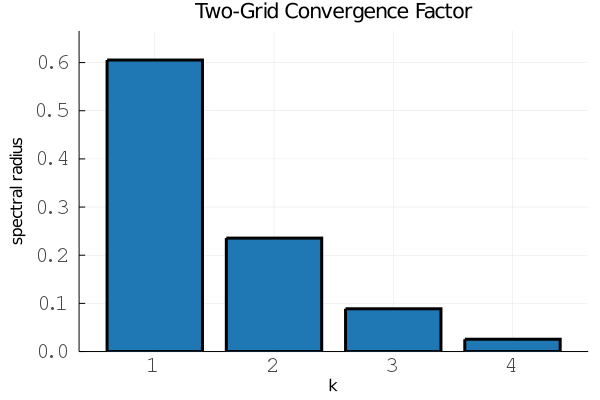
\includegraphics[width=0.48\textwidth]{img/two_grid_converge_5_to_3_chebyshev}\label{fig:two_grid_5_3_chebyshev}}
    \subfloat[Convergence for $p = 4$ to $p = 1$, $\nu = 1$]{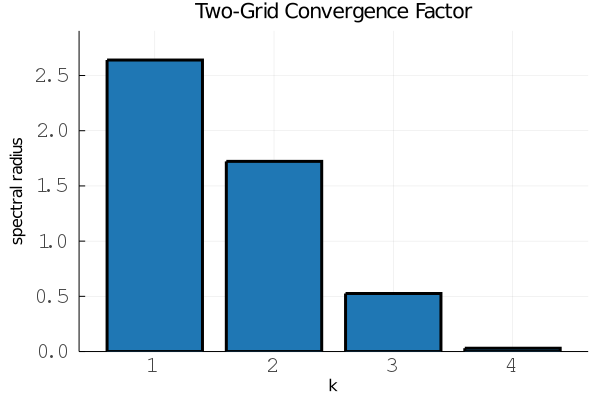
\includegraphics[width=0.48\textwidth]{img/two_grid_converge_5_to_2_chebyshev}\label{fig:two_grid_5_2_chebyshev}}
  \caption{Two-grid analysis for Chebyshev smoothing for high-order finite elements}
\end{figure}

In Figures \ref{fig:two_grid_5_3_chebyshev} and \ref{fig:two_grid_5_2_chebyshev} we plot the two-grid convergence factor for p-multigrid with Chebyshev pre and post-smoothing for the one dimensional Laplacian as a function of the Chebyshev order, $\omega$.
On the left we show conservative coarsening from quartic to quadratic elements and on the right we show more aggressive coarsening from quartic to linear elements.
As expected, the two-grid convergence factor decreases as we coarsen more rapidly, however this effect is not as pronounced as we saw with Jacobi smoothing.

% -----------------------------------------------------------------------------
\subsection{Scalar Laplacian - 2D Convergence Factors}\label{sec:2dresults}
% -----------------------------------------------------------------------------

\subsubsection{Jacobi Smoothing}
% -----------------------------------------------------------------------------

Figures \ref{fig:jacobi_smooth_factor_2d} and \ref{fig:two_grid_5_to_3_2d} show the Jacobi smoothing factor and two-grid convergence factor for p-multigrid with one iteration of Jacobi smoothing for the two dimensional Laplacian as a function of the Jacobi smoothing parameter $\omega$.
Again, the Jacobi smoothing factor is a poor predictor for the two-grid smoothing factor.

\begin{figure}[!tbp]
  \centering
  \subfloat[Smoothing Factor of 2D Jacobi for $p = 4$]{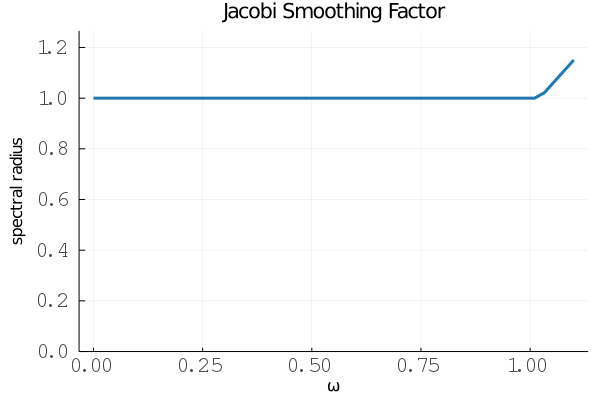
\includegraphics[width=0.48\textwidth]{img/jacobi_smoothing_5_2d}\label{fig:jacobi_smooth_factor_2d}}
  \hfill
  \subfloat[Convergence for $p = 4$ to $p = 2$, $\nu = 1$]{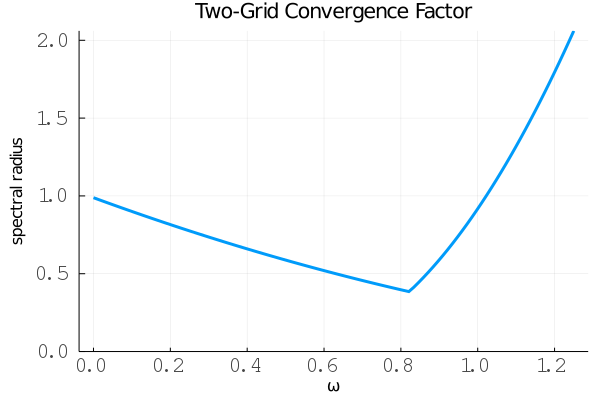
\includegraphics[width=0.48\textwidth]{img/two_grid_converge_5_to_3_2d}\label{fig:two_grid_5_to_3_2d}}
  \caption{Convergence for 2D high-order finite elements}
\end{figure}

\begin{table}[ht!]
\begin{center}
\begin{tabular}{l cc cc cc}
  \toprule
  $p_{\text{fine}}$ to $p_{\text{coarse}}$  &  \multicolumn{2}{c}{$\nu = 1$}            &  \multicolumn{2}{c}{$\nu = 2$}         &  \multicolumn{2}{c}{$\nu = 3$}           \\
  %\cmidrule(lr){2-3} \cmidrule(lr){4-5} \cmidrule(lr){6-7}
                                            &  $\rho_{\min}$  &  $\omega_{\text{opt}}$  &  $\rho_{\min}$ & $\omega_{\text{opt}}$  &  $\rho_{\min}$ & $\omega_{\text{opt}}$  \\
  \midrule
  $p = 2$ to $p = 1$          &  0.229 & 0.952  &  0.091 & 0.997  &  0.062 & 1.000   \\
  %\midrule
  $p = 4$ to $p = 2$          &  0.385 & 0.826  &  0.149 & 0.824  &  0.077 & 0.838   \\
  $p = 4$ to $p = 1$          &  0.761 & 0.958  &  0.580 & 0.958  &  0.441 & 0.958   \\
  %\midrule
  $p = 8$ to $p = 4$          &  0.644 & 0.794  &  0.416 & 0.794  &  0.270 & 0.825   \\
  $p = 8$ to $p = 2$          &  0.857 & 0.848  &  0.735 & 0.848  &  0.630 & 0.848   \\
  $p = 8$ to $p = 1$          &  0.952 & 0.871  &  0.907 & 0.871  &  0.864 & 0.871   \\
  \bottomrule
\end{tabular}
\end{center}
\caption{Two-grid smoothing factor and optimal Jacobi parameter for 2D Laplacian}
\label{table:two_grid_2d}
\end{table}

The results in Table \ref{table:two_grid_2d} provide the minimal LFA smoothing factor and optimal values of $\omega$ for two-grid high-order p-multigrid for a variety of polynomial orders and coarsening factors.

\begin{figure}[!tbp]
  \centering
    \subfloat[Spectral radius for $p = 8$ to $p = 1$, $\nu = 3$]{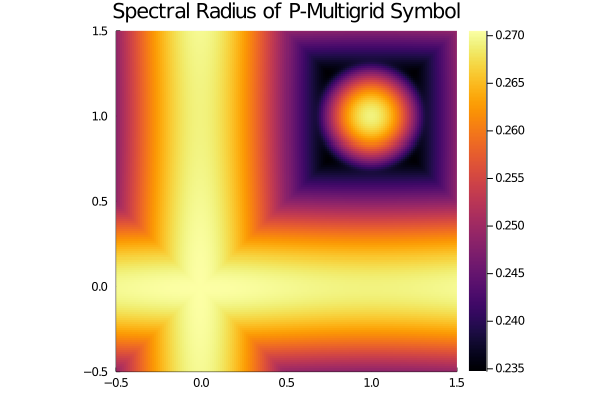
\includegraphics[width=0.48\textwidth]{img/multi_grid_spectral_radius_9_to_2_2d}\label{fig:multi_grid_spectral_radius_9_2_2d}}
    \subfloat[Convergence for $p = 8$ to $p = 1$, $\nu = 3$]{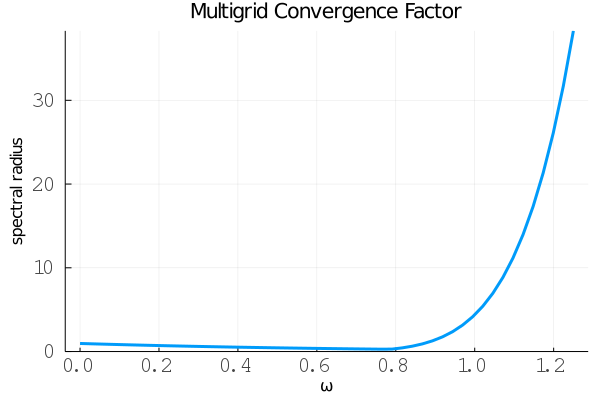
\includegraphics[width=0.48\textwidth]{img/multi_grid_converge_9_to_2_3smooth_2d}\label{fig:multi_grid_9_2_3smooth_2d}}
  \caption{Multigrid analysis for Jacobi smoothing for 2D high-order finite elements}
\end{figure}

In Figures \ref{fig:multi_grid_spectral_radius_9_2_2d} and \ref{fig:multi_grid_9_2_2smooth_2d} we plot the spectral radius of the multigrid symbol and multigrid convergence factor for p-multigrid with three iterations of Jacobi pre and post-smoothing for the two dimensional Laplacian.

\subsubsection{Chebyshev Smoothing}
% -----------------------------------------------------------------------------

% -----------------------------------------------------------------------------
\subsection{Neo-Hookean Hyperelasticity - 3D Convergence Factors}\label{sec:3dresults}
% -----------------------------------------------------------------------------

% -----------------------------------------------------------------------------
\section{Conclusions}\label{sec:conclusion}
% -----------------------------------------------------------------------------

In this paper we introduced LFAToolkit.jl \cite{thompson2021toolkit}, a new Julia package for LFA of high-order finite element methods.
Specifically, we developed LFA of p-multigrid with arbitrary second-order PDEs using high-order finite element discretizations and investigated Jacobi smoothing for p-multigrid with LFAToolkit.jl.

Traditional estimates of the optimal Jacobi smoothing parameter are ill-suited to p-multigrid for the one and two dimensional Laplacian discretized with high-order finite elements, but analysis of the two-grid smoothing factor can provide a reasonable underestimate of the optimal Jacobi smoothing parameter for multigrid schemes.

% -----------------------------------------------------------------------------
\bibliographystyle{siamplain}
\bibliography{references}
% -----------------------------------------------------------------------------

\end{document}

% -----------------------------------------------------------------------------
